\documentclass[margin=10pt]{standalone}
\usepackage{color,xcolor}
\usepackage{makecell}
\usepackage{tikz-qtree, tikz}
\usepackage[utf8]{inputenc}

\definecolor{myblue}{HTML}{0072BD}
\definecolor{mygreen}{HTML}{258F1B}
\definecolor{myred}{HTML}{C4000C}

\usetikzlibrary{decorations.pathreplacing,arrows,shapes,positioning,shadows,calc}
\usetikzlibrary{decorations, decorations.text,backgrounds}
\tikzset{every picture/.style={font issue=\footnotesize},
    font issue/.style={execute at begin picture={#1\selectfont}}
}
\newcommand{\tick}{\tikz \draw[-,ultra thick] (0,-0.75) -- +(0,0.75);}

\begin{document}
\begin{tikzpicture}
% [every node/.style={inner sep=0,outer sep=60}]
    \node[anchor=south west,scale=0.5,outer sep=60] (twM1) at (0,0) {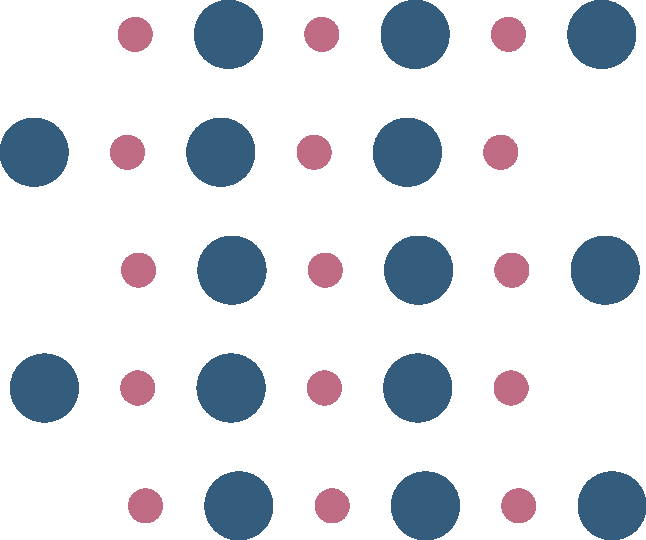
\includegraphics{twinned-martensite-phase.pdf}};
    \node[anchor=south west,scale=0.5,outer sep=60] (A1) at (15,0) {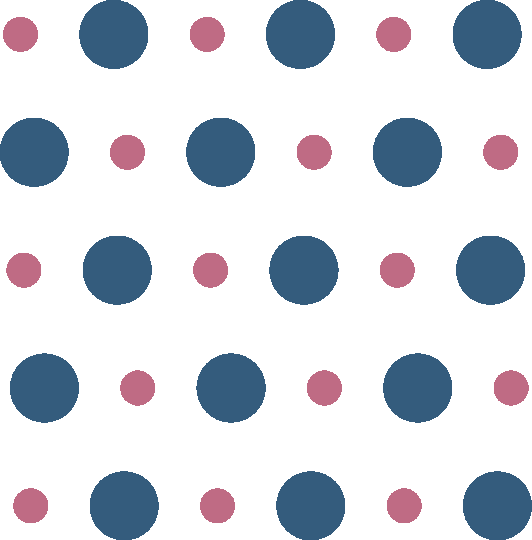
\includegraphics{austenite-phase.pdf}};
    \node[anchor=south west,scale=0.5,outer sep=60] (twM2) at (0,8) {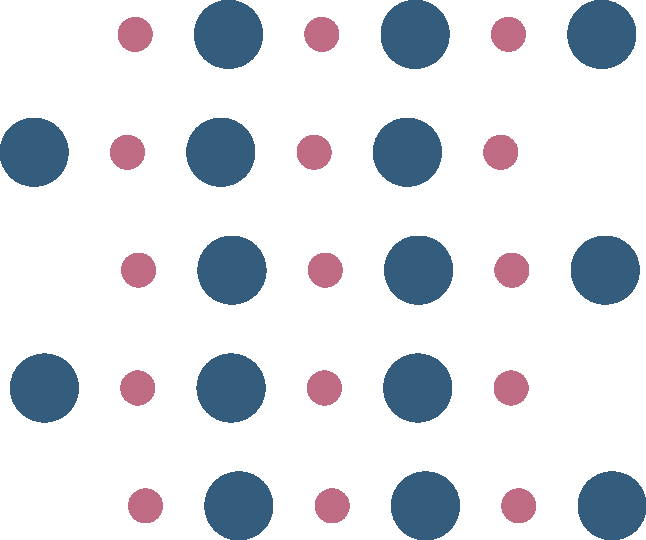
\includegraphics{twinned-martensite-phase.pdf}};
    \node[anchor=south west,scale=0.5,outer sep=60] (A2) at (15,8) {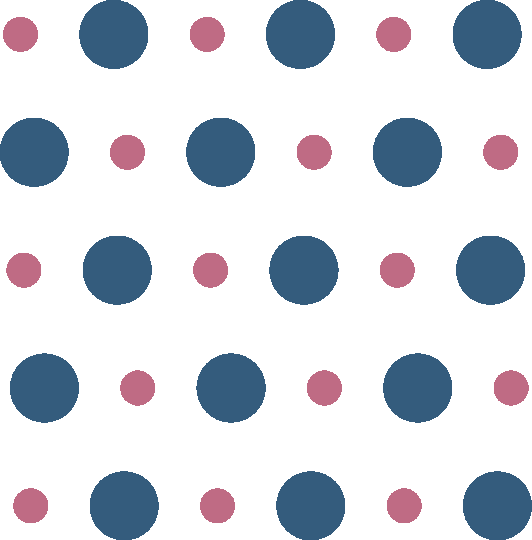
\includegraphics{austenite-phase.pdf}};

    \node[anchor=center,yshift=50] (A1text)[below = of A1] {\Large Austenite};
    \node[anchor=center,yshift=50] (A2text)[below = of A2] {\Large Austenite};
    \node[anchor=center,yshift=50] (twM1text)[below = of twM1] {\Large Twinned Martensite};
    \node[anchor=center,yshift=50] (twM2text)[below = of twM2] {\Large Twinned Martensite};

    % Axes with ticks
    \draw [-latex,ultra thick] (0,7.5) -- node[pos=0.325] {\tick} node[pos=0.4] {\tick} node[pos=0.6] {\tick} node[pos=0.6,yshift=-30] {\huge $A_s$} node[pos=0.675] {\tick} node[pos=0.675,yshift=-30] {\huge $A_f$} node[pos=1,yshift=-25] {\huge$T$} (22,7.5);
    \draw [-latex,ultra thick] (0,-0.25) -- node[pos=0.325] {\tick} node[pos=0.325,yshift=-30] {\huge $M_f$} node[pos=0.4] {\tick} node[pos=0.4,yshift=-30] {\huge $M_s$} node[pos=0.6] {\tick} node[pos=0.675] {\tick} node[pos=1,yshift=-25] {\huge$T$} (22,-0.25);
    % Phase transformations arrow and labels
    \draw [-latex,ultra thick,color=myblue] (A1.west) -- node [midway,above,outer sep=10,color=myblue] {\Huge$T\downarrow$} node [midway,below,outer sep=10,color=black] {\Huge$M\leftarrow A$} (twM1.east);
    \draw [-latex,ultra thick,color=myred] (twM2.east) -- node [midway,above,outer sep=10,color=myred] {\Huge$T\uparrow$} node [midway,below,outer sep=10,color=black] {\Huge$M\rightarrow A$} (A2.west);
\end{tikzpicture}
\end{document}
